\documentclass[a4paper, 12pt]{article}

\usepackage{iftex}
\ifPDFTeX
    % pdfLaTeX: кириллица через T2A
    \usepackage[T1, T2A]{fontenc}
    \usepackage[utf8]{inputenc}
    \usepackage[english, russian]{babel}
\else
    % XeLaTeX / LuaLaTeX: нужен шрифт с кириллицей (берём первый найденный)
    \usepackage{fontspec}
    \usepackage[english, russian]{babel}
    % Windows/macOS: Times New Roman и Courier New; Linux: Liberation или DejaVu
    \IfFontExistsTF{Times New Roman}{\setmainfont{Times New Roman}}{%
    \IfFontExistsTF{Liberation Serif}{\setmainfont{Liberation Serif}}{%
    \setmainfont{DejaVu Serif}}}
    \IfFontExistsTF{Courier New}{\setmonofont{Courier New}}{%
    \IfFontExistsTF{Liberation Mono}{\setmonofont{Liberation Mono}}{%
    \setmonofont{DejaVu Sans Mono}}}
\fi
\usepackage{graphicx}
\usepackage{float}
\usepackage{geometry}
\usepackage{amsmath}
\usepackage{amsfonts}
\usepackage{booktabs}
\usepackage[dvipsnames]{xcolor}
\usepackage[colorlinks]{hyperref}
\usepackage{indentfirst}
\usepackage{listings}
\usepackage{src/title}

\geometry{left=2cm, right=2cm, bottom=2cm, top=2cm}

\hypersetup{
    linkcolor=blue,
    filecolor=magenta,
    urlcolor=cyan
}

\definecolor{codegreen}{rgb}{0,0.6,0}
\definecolor{codegray}{rgb}{0.5,0.5,0.5}
\definecolor{codepurple}{rgb}{0.58,0,0.82}
\definecolor{backcolour}{rgb}{0.95,0.95,0.92}

\lstdefinestyle{codestyle}{
    backgroundcolor=\color{backcolour},
    commentstyle=\color{codegreen},
    keywordstyle=\color{magenta},
    numberstyle=\tiny\color{codegray},
    stringstyle=\color{codepurple},
    basicstyle=\ttfamily\footnotesize,
    breakatwhitespace=false,
    breaklines=true,
    captionpos=b,
    keepspaces=true,
    numbers=left,
    numbersep=5pt,
    showspaces=false,
    showstringspaces=false,
    showtabs=false,
    tabsize=2
}
\lstset{style=codestyle}
\lstset{extendedchars=\true}

\setlength{\emergencystretch}{3em}
\DeclareMathOperator{\rank}{rank}
\DeclareMathOperator{\tr}{tr}
\newcommand{\hv}{\hat v}

% Числовые матрицы: файл создаётся программой prog/main.py
% Файл создаётся автоматически программой prog/main.py — не править вручную
\newcommand{\MatSa}{\begin{pmatrix}2 & 0 & 0 & 0 \\ 0 & 1 & 0 & 0 \\ 0 & 0 & 1.5 & 0 \\ 0 & 0 & 0 & 1\end{pmatrix}}
\newcommand{\MatSb}{\begin{pmatrix}0.5 & 0 & 0 & 0 \\ 0 & 2 & 0 & 0 \\ 0 & 0 & 2 & 0 \\ 0 & 0 & 0 & 1\end{pmatrix}}
\newcommand{\MatSab}{\begin{pmatrix}1 & 0 & 0 & 0 \\ 0 & 2 & 0 & 0 \\ 0 & 0 & 3 & 0 \\ 0 & 0 & 0 & 1\end{pmatrix}}
\newcommand{\MatTa}{\begin{pmatrix}1 & 0 & 0 & 2 \\ 0 & 1 & 0 & 1 \\ 0 & 0 & 1 & 0 \\ 0 & 0 & 0 & 1\end{pmatrix}}
\newcommand{\MatTb}{\begin{pmatrix}1 & 0 & 0 & -1 \\ 0 & 1 & 0 & 0 \\ 0 & 0 & 1 & 2 \\ 0 & 0 & 0 & 1\end{pmatrix}}
\newcommand{\MatTab}{\begin{pmatrix}1 & 0 & 0 & 1 \\ 0 & 1 & 0 & 1 \\ 0 & 0 & 1 & 2 \\ 0 & 0 & 0 & 1\end{pmatrix}}
\newcommand{\MatTS}{\begin{pmatrix}1 & 0 & 0 & 1 \\ 0 & 2 & 0 & 1 \\ 0 & 0 & 3 & 2 \\ 0 & 0 & 0 & 1\end{pmatrix}}
\newcommand{\MatST}{\begin{pmatrix}1 & 0 & 0 & 1 \\ 0 & 2 & 0 & 2 \\ 0 & 0 & 3 & 6 \\ 0 & 0 & 0 & 1\end{pmatrix}}
\newcommand{\MatJa}{\begin{pmatrix}0 & -0.6667 & 0.6667 \\ 0.6667 & 0 & -0.3333 \\ -0.6667 & 0.3333 & 0\end{pmatrix}}
\newcommand{\MatRa}{\begin{pmatrix}0.5556 & -0.4662 & 0.6885 & 0 \\ 0.6885 & 0.7222 & -0.0665 & 0 \\ -0.4662 & 0.5109 & 0.7222 & 0 \\ 0 & 0 & 0 & 1\end{pmatrix}}
\newcommand{\MatRb}{\begin{pmatrix}0.8373 & -0.5365 & -0.1055 & 0 \\ 0.4063 & 0.7397 & -0.5365 & 0 \\ 0.3659 & 0.4063 & 0.8373 & 0 \\ 0 & 0 & 0 & 1\end{pmatrix}}
\newcommand{\MatRba}{\begin{pmatrix}0.145 & -0.8318 & 0.5359 & 0 \\ 0.9851 & 0.0707 & -0.1569 & 0 \\ 0.0926 & 0.5506 & 0.8296 & 0 \\ 0 & 0 & 0 & 1\end{pmatrix}}
\newcommand{\MatRab}{\begin{pmatrix}0.5276 & -0.3632 & 0.7679 & 0 \\ 0.8456 & 0.1378 & -0.5158 & 0 \\ 0.0815 & 0.9215 & 0.3798 & 0 \\ 0 & 0 & 0 & 1\end{pmatrix}}
\newcommand{\AxisBA}{\begin{pmatrix}0.354 \\ 0.222 \\ 0.909\end{pmatrix}}
\newcommand{\AxisAB}{\begin{pmatrix}0.719 \\ 0.343 \\ 0.605\end{pmatrix}}
\newcommand{\AngleBA}{88.7}
\newcommand{\AngleAB}{88.7}
\newcommand{\MatRvertex}{\begin{pmatrix}0.75 & 0.25 & 0.6124 & -0.6124 \\ 0.25 & 0.75 & -0.6124 & 0.6124 \\ -0.6124 & 0.6124 & 0.5 & 0.5 \\ 0 & 0 & 0 & 1\end{pmatrix}}
\newcommand{\MatRc}{\begin{pmatrix}0.866 & 0.2113 & 0.4532 & 0 \\ 0 & 0.9063 & -0.4226 & 0 \\ -0.5 & 0.366 & 0.7849 & 0 \\ 0 & 0 & 0 & 1\end{pmatrix}}
\newcommand{\MatTc}{\begin{pmatrix}1 & 0 & 0 & -5.438 \\ 0 & 1 & 0 & 5.071 \\ 0 & 0 & 1 & -9.419 \\ 0 & 0 & 0 & 1\end{pmatrix}}
\newcommand{\MatC}{\begin{pmatrix}0.866 & 0.2113 & 0.4532 & -5.4378 \\ 0 & 0.9063 & -0.4226 & 5.0714 \\ -0.5 & 0.366 & 0.7849 & -9.4186 \\ 0 & 0 & 0 & 1\end{pmatrix}}
\newcommand{\MatCinv}{\begin{pmatrix}0.866 & 0 & -0.5 & 0 \\ 0.2113 & 0.9063 & 0.366 & 0 \\ 0.4532 & -0.4226 & 0.7849 & 12 \\ 0 & 0 & 0 & 1\end{pmatrix}}
\newcommand{\CamPos}{\begin{pmatrix}-5.438 \\ 5.071 \\ -9.419\end{pmatrix}}
\newcommand{\MatP}{\begin{pmatrix}1.7321 & 0 & 0 & 0 \\ 0 & 1.7321 & 0 & 0 \\ 0 & 0 & 1.5 & -12.5 \\ 0 & 0 & 1 & 0\end{pmatrix}}
\newcommand{\ZRange}{7.32\ldots 14.79}
\newcommand{\NDCmax}{0.883}
\newcommand{\MatCh}{\begin{pmatrix}0.807 & -0.249 & 0.535 & -9 \\ -0.59 & -0.341 & 0.732 & -13 \\ 0 & -0.906 & -0.422 & 9 \\ 0 & 0 & 0 & 1\end{pmatrix}}
\newcommand{\MatPh}{\begin{pmatrix}1.732 & 0 & 0 & 0 \\ 0 & 1.732 & 0 & 0 \\ 0 & 0 & 1.286 & -11.429 \\ 0 & 0 & 1 & 0\end{pmatrix}}


\title{
    Практическая линейная алгебра — Лабораторная работа №3
}

\author{%
    Ануфриев Андрей Сергеевич (465029)\\
    Бахуров Николай Алексеевич (504862)\\
    Раджапов Фёдор Сергеевич (502544)%
}

\supervisor{Зарина Ольга Андреевна}

\abstract{
    В работе исследованы матрицы $4\times4$ в однородных координатах, применяемые в 3D-графике. Построены матрицы масштабирования, перемещения и поворота (по формуле $R_v(\theta)=e^{J\theta}$), поворота вокруг оси через заданную точку, матрицы положения камеры и перспективы. Все преобразования выполнены матричным умножением над вершинами кубика и сцены из нескольких фигур, результаты визуализированы на Python (\texttt{matplotlib}), выполнено необязательное задание~8 (домик).
}

\keywords{
    однородные координаты; матрицы преобразований; поворот; матричная экспонента; камера; перспектива
}

\date{2026-10-29}

\begin{document}
    \maketitle
    \tableofcontents
    \newpage

    \section{Постановка задачи}
    Требуется познакомиться с матрицами преобразований пространства в однородных координатах и построить с их помощью: куб и другую фигуру (задание~1), масштабирование (2), перемещение (3), поворот вокруг оси $v$ через начало координат (4) и вокруг вершины куба (5), камеру (6) и перспективу (7), а также домик из блоков (8, необязательное). Все преобразования координат выполняются \emph{только} матричным умножением.

    \textbf{Соглашения.} Точка $p=(x,y,z)$ записывается столбцом $(x,y,z,1)^T$, преобразование --- левое умножение $p'=Mp$. Композиция «сначала $A$, затем $B$» равна $BA$. (В одном из источников методички матрицы транспонированы, т.\,е. используются векторы-строки: $p'=pM^T$.) Камера по умолчанию находится в начале координат и смотрит вдоль $+z$, ось $x$ направлена вправо, ось $y$ --- вниз; так выглядит график при \texttt{ax.view\_init(azim=0, elev=-90)} (при необходимости с \texttt{roll=-90}, см. задание~6).

    Все числовые матрицы в тексте подставляются из файла \texttt{matrices.tex}, который создаёт программа, поэтому числа в отчёте совпадают с расчётом в коде.

    \section{Задание 1. Куб}
    Куб задан матрицей вершин $4\times8$ (столбец --- вершина) и списком граней (номера вершин, нумерация с нуля), как в листинге методички:
    $$V_{cube}=\begin{pmatrix}-1&1&1&-1&-1&1&1&-1\\-1&-1&1&1&-1&-1&1&1\\-1&-1&-1&-1&1&1&1&1\\1&1&1&1&1&1&1&1\end{pmatrix}.$$
    Функция \texttt{draw\_shape} берёт первые три строки и делит их на четвёртую: $(x,y,z,w)\mapsto(x/w,y/w,z/w)$, затем строит многоугольники по спискам индексов граней.

    \textbf{Почему четыре компоненты, а не три.} Перемещение $p\mapsto p+t$ не является линейным отображением $\mathbb R^3$ (нулевой вектор не остаётся нулевым), поэтому его нельзя записать матрицей $3\times3$. В однородных координатах $(x,y,z,1)$ оно становится линейным: $\begin{pmatrix}I&t\\0&1\end{pmatrix}\begin{pmatrix}p\\1\end{pmatrix}=\begin{pmatrix}p+t\\1\end{pmatrix}$. Благодаря этому масштабирование, поворот, перемещение и перспектива --- матрицы одного размера, и любую цепочку преобразований можно заранее перемножить в одну матрицу. Четвёртая компонента $w\neq1$ нужна для перспективы (деление на $w$). Векторы с $w=0$ описывают направления (точки на бесконечности), к ним перемещение не применяется.

    \textbf{Как задать другую фигуру.} Нужно заменить матрицу вершин $4\times N$ и список граней: каждая грань --- список номеров вершин в порядке обхода (длины граней могут быть разными). Для пирамиды с квадратным основанием:
    $$V_{pyr}=\begin{pmatrix}-1&1&1&-1&0\\-1&-1&1&1&0\\-1&-1&-1&-1&1\\1&1&1&1&1\end{pmatrix},\quad
    \text{грани: }[0,1,2,3],\ [0,1,4],\ [1,2,4],\ [2,3,4],\ [3,0,4].$$
    \begin{figure}[H]
        \centering
        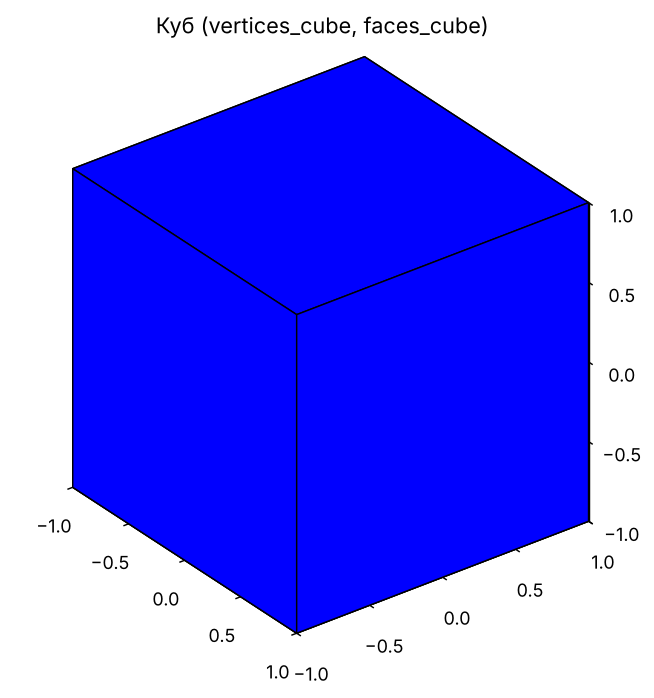
\includegraphics[width=0.48\textwidth]{../graphics/t1_cube.png}\hfill
        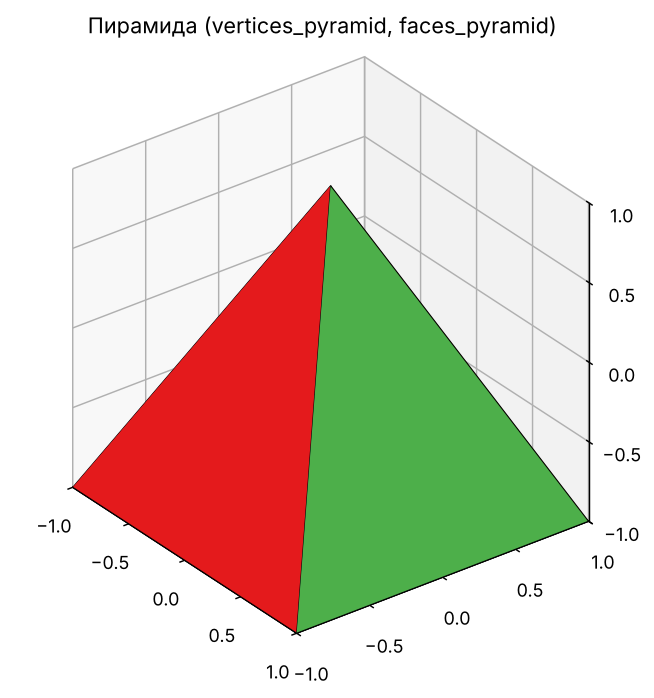
\includegraphics[width=0.48\textwidth]{../graphics/t1_pyramid.png}
        \caption{Задание 1. Результат программы для куба (слева) и для пирамиды (справа)}
        \label{fig:t1}
    \end{figure}

    \section{Задание 2. Масштабирование}
    \textbf{Общая структура.} Масштабирование по осям с коэффициентами $s_x,s_y,s_z$ (центр --- начало координат):
    $$S(s_x,s_y,s_z)=\begin{pmatrix}s_x&0&0&0\\0&s_y&0&0\\0&0&s_z&0\\0&0&0&1\end{pmatrix},\qquad \det S=s_xs_ys_z.$$
    Объём изменяется в $|s_xs_ys_z|$ раз; $s_i<0$ даёт ещё и отражение; $S^{-1}=S(1/s_x,1/s_y,1/s_z)$. Композиция двух масштабирований --- снова масштабирование с произведением коэффициентов: $S(a)S(b)=S(a_xb_x,a_yb_y,a_zb_z)$.

    \textbf{Выбранные матрицы.}
    \begin{gather*}
    S_1=S(2,1,1.5)=\MatSa,\quad S_2=S(0.5,2,2)=\MatSb,\\
    S_2S_1=\MatSab=S(1,2,3).
    \end{gather*}
    Куб растягивается вдоль $x$ и $z$ (для $S_1$), вдоль $y$ и $z$ с одновременным сжатием вдоль $x$ (для $S_2$); итоговая матрица оставляет размер по $x$ равным 2, удваивает по $y$ и утраивает по $z$. Центр куба остаётся в начале координат (на рисунке серым показан исходный куб).
    \begin{figure}[H]
        \centering
        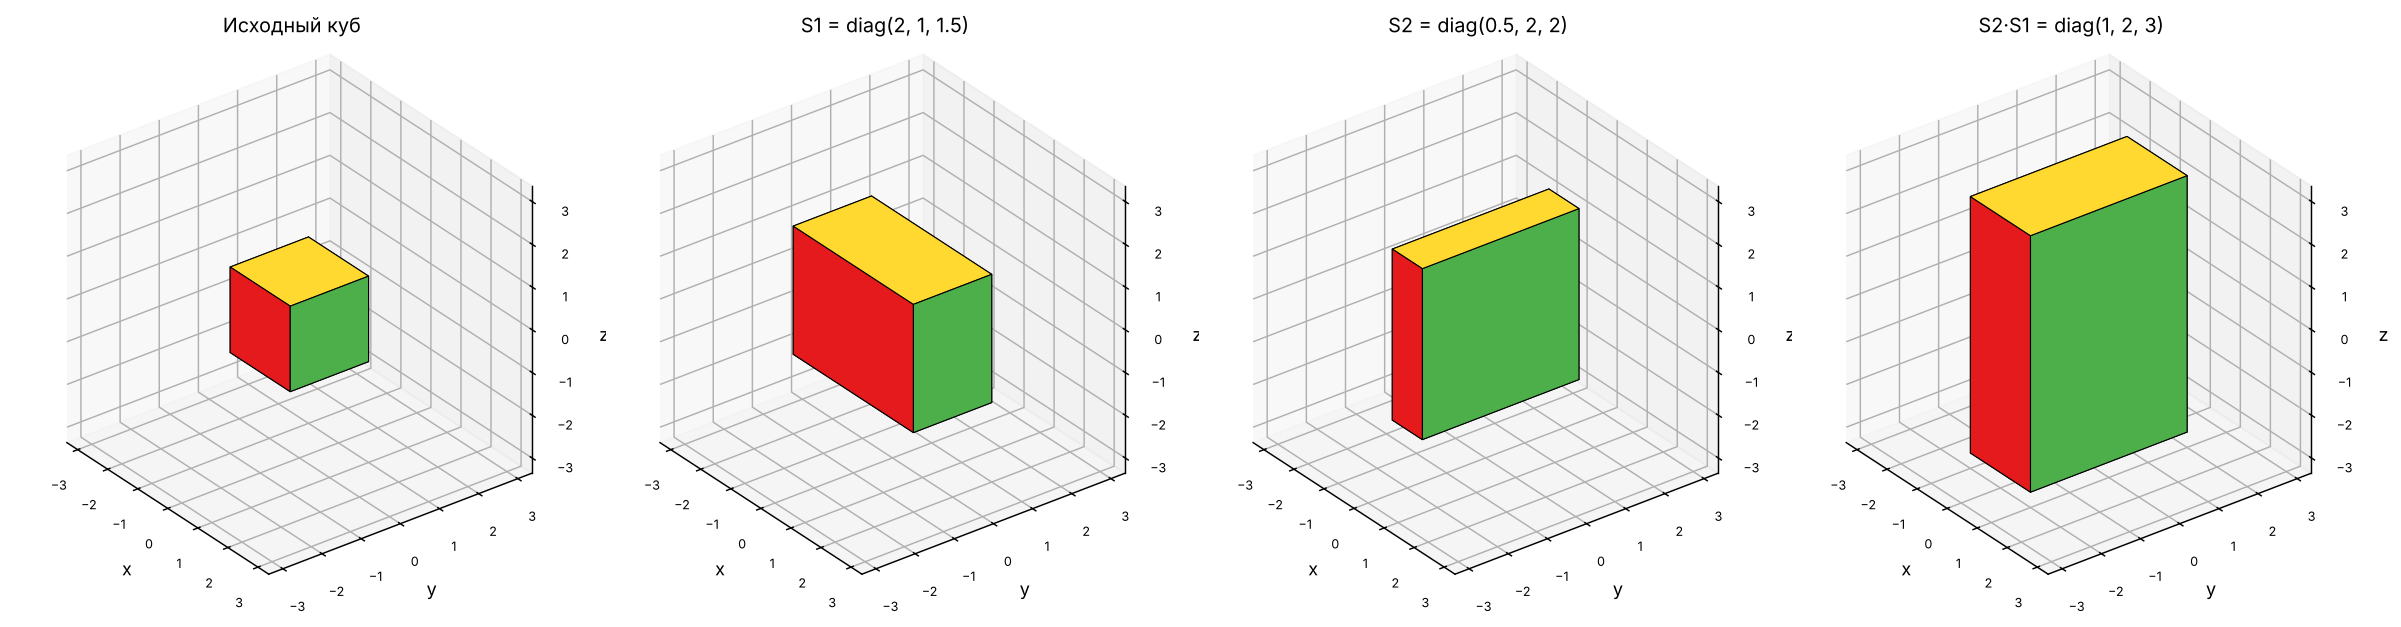
\includegraphics[width=\textwidth]{../graphics/t2_scale.png}
        \caption{Задание 2. Исходный куб, образы под действием $S_1$, $S_2$ и $S_2S_1$}
        \label{fig:t2}
    \end{figure}

    \section{Задание 3. Перемещение}
    \textbf{Общая структура.} Перемещение на вектор $t=(t_x,t_y,t_z)^T$:
    $$T(t_x,t_y,t_z)=\begin{pmatrix}1&0&0&t_x\\0&1&0&t_y\\0&0&1&t_z\\0&0&0&1\end{pmatrix}=\begin{pmatrix}I&t\\0&1\end{pmatrix}.$$
    Действие: $T(x,y,z,1)^T=(x+t_x,y+t_y,z+t_z,1)^T$. Свойства: $T(a)T(b)=T(a+b)$, $T(t)^{-1}=T(-t)$, $\det T=1$ (объём сохраняется), $T$ не является линейным отображением $\mathbb R^3$, а лишь аффинным.

    \textbf{Выбранные матрицы.}
    \begin{gather*}
    T_1=T(2,1,0)=\MatTa,\quad T_2=T(-1,0,2)=\MatTb,\\
    T_2T_1=T(1,1,2)=\MatTab.
    \end{gather*}
    \begin{figure}[H]
        \centering
        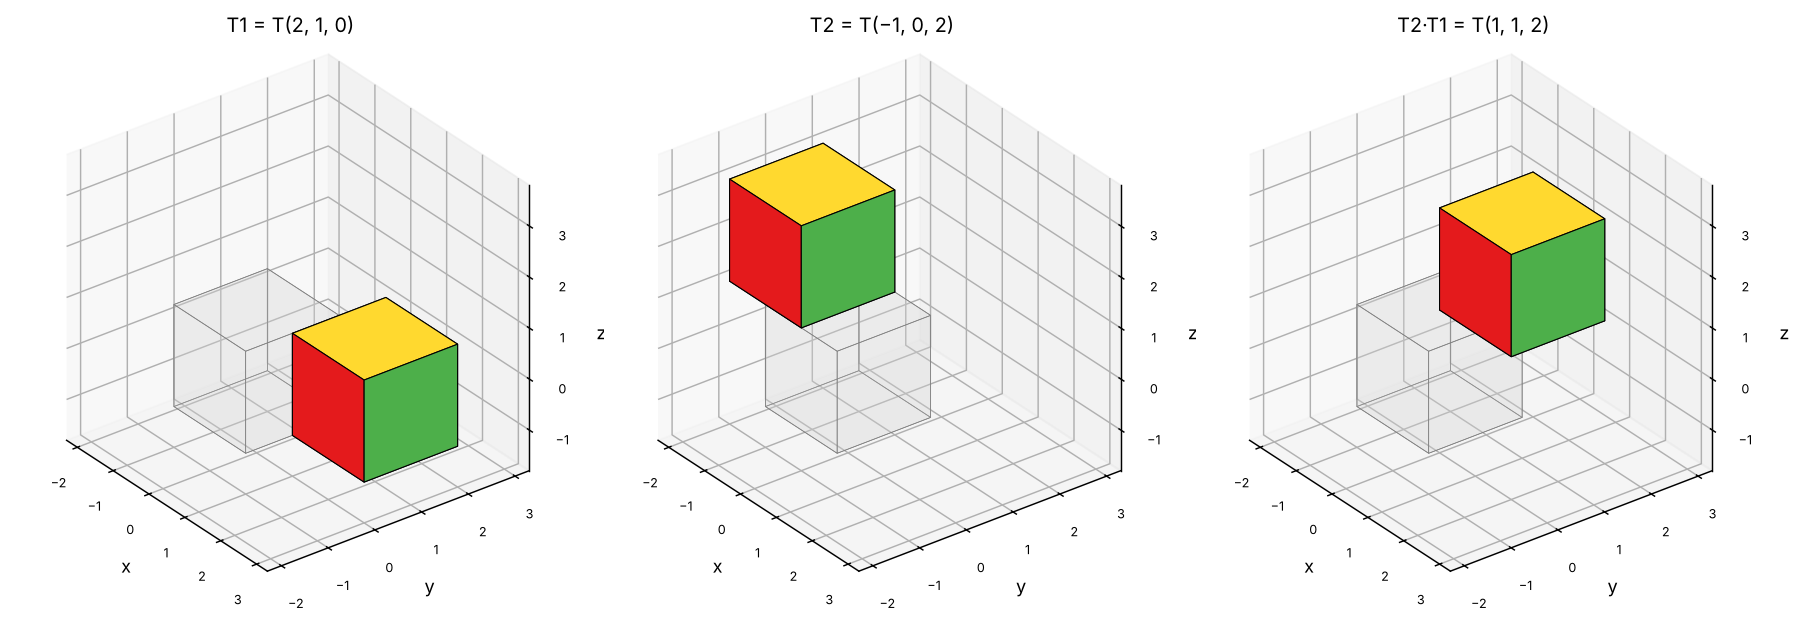
\includegraphics[width=\textwidth]{../graphics/t3_translate.png}
        \caption{Задание 3. Образы куба под действием $T_1$, $T_2$ и $T_2T_1$}
        \label{fig:t3}
    \end{figure}

    \textbf{Комбинации $TS$ и $ST$.} Пусть $S=S_2S_1=\mathrm{diag}(1,2,3,1)$ и $T=T_2T_1=T(1,1,2)$. В блочном виде
    $$TS=\begin{pmatrix}I&t\\0&1\end{pmatrix}\begin{pmatrix}S&0\\0&1\end{pmatrix}=\begin{pmatrix}S&t\\0&1\end{pmatrix},\qquad
    ST=\begin{pmatrix}S&0\\0&1\end{pmatrix}\begin{pmatrix}I&t\\0&1\end{pmatrix}=\begin{pmatrix}S&St\\0&1\end{pmatrix}.$$
    Численно:
    $$TS=\MatTS,\qquad ST=\MatST.$$
    Преобразования \textbf{не эквивалентны}: $TS=ST\iff St=t\iff (S-I)t=0$. Здесь $St=(1,2,6)^T\neq t=(1,1,2)^T$. Геометрически: в $TS$ куб сначала растягивается вокруг своего центра, затем сдвигается на $t$ (центр оказывается в $(1,1,2)$); в $ST$ куб сначала сдвигается, а затем вместе со сдвигом растягивается относительно начала координат --- сдвиг тоже масштабируется (центр оказывается в $St=(1,2,6)$).
    \begin{figure}[H]
        \centering
        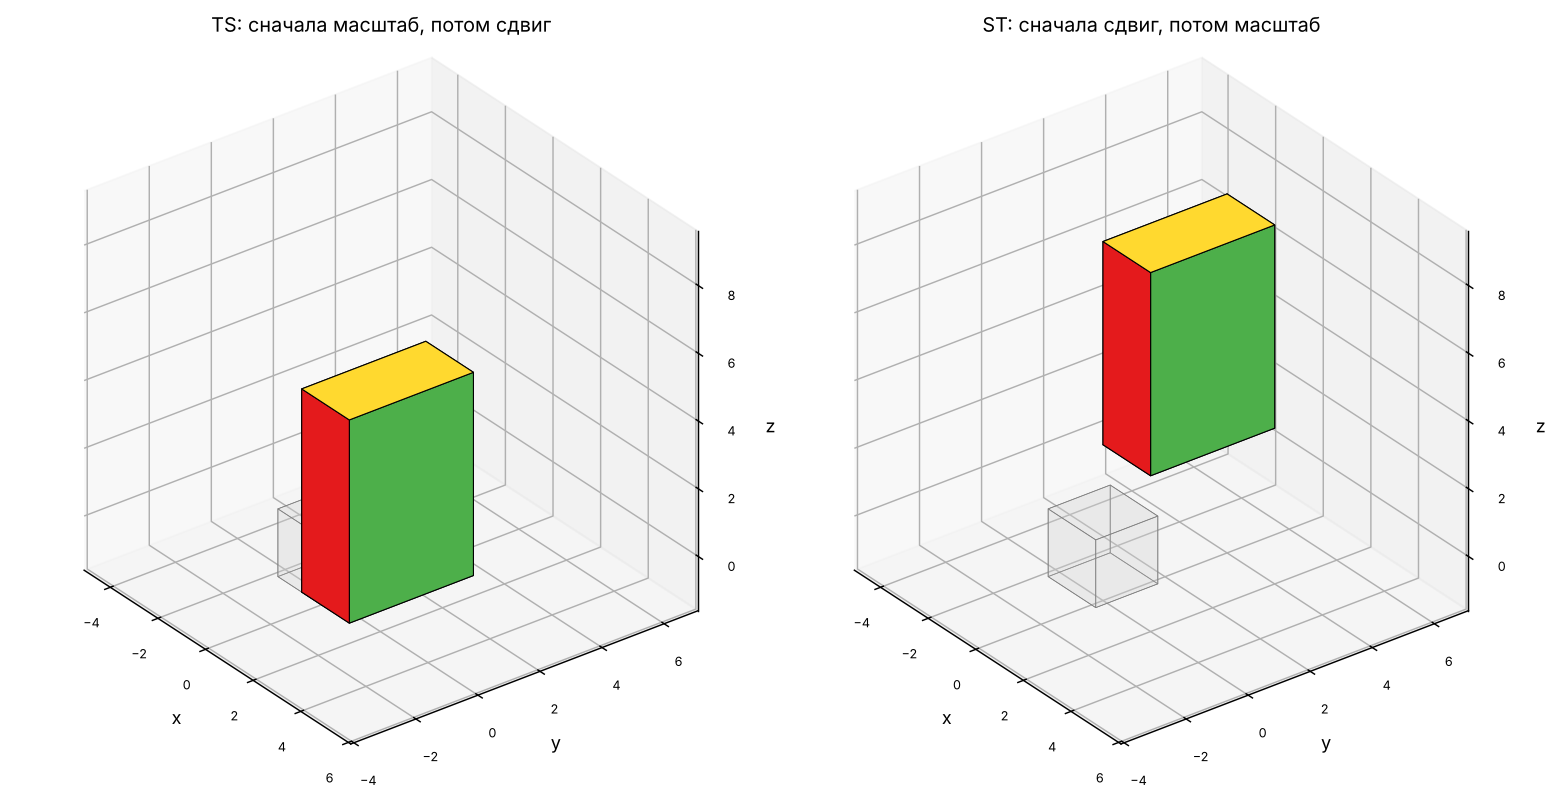
\includegraphics[width=\textwidth]{../graphics/t3_TS_ST.png}
        \caption{Задание 3. Слева $TS$ (масштаб, затем сдвиг), справа $ST$ (сдвиг, затем масштаб)}
        \label{fig:t3ts}
    \end{figure}

    \section{Задание 4. Вращение вокруг оси}
    \textbf{Общая структура.} Пусть $v=(v_x,v_y,v_z)^T$ --- ось вращения (через начало координат), $\hv=v/\|v\|$. Матрица
    $$J=\begin{pmatrix}0&-\hat v_z&\hat v_y&0\\ \hat v_z&0&-\hat v_x&0\\ -\hat v_y&\hat v_x&0&0\\0&0&0&0\end{pmatrix}$$
    --- кососимметрическая матрица векторного произведения: для любого $w$ верно $Jw=\hv\times w$. Поворот на угол $\theta$ против часовой стрелки (если смотреть с конца вектора $\hv$): $R_v(\theta)=e^{J\theta}$.

    \textbf{Как работает формула.} Функция $\varphi(\theta)=e^{J\theta}p$ --- решение уравнения $\dot x=Jx=\hv\times x$, то есть движения точки с угловой скоростью $\hv$ (вращение вокруг $\hv$ с единичной угловой скоростью), поэтому $e^{J\theta}$ поворачивает на угол $\theta$. Для $\|\hv\|=1$ выполнено $J^2=\hv\hv^T-I$ и $J^3=-J$ (на блоке $3\times3$), поэтому ряд $e^{J\theta}=\sum J^k\theta^k/k!$ сворачивается в формулу Родрига
    $$R_v(\theta)=I+\sin\theta\,J+(1-\cos\theta)J^2,\qquad\text{на блоке }3\times3:\ \cos\theta\,I+\sin\theta\,J+(1-\cos\theta)\hv\hv^T.$$
    Ось неподвижна: $J\hv=\hv\times\hv=0$, поэтому $e^{J\theta}\hv=\hv$. Матрица $R$ ортогональна, так как $J^T=-J$ и $(e^{J\theta})^T=e^{-J\theta}=(e^{J\theta})^{-1}$, а $\det e^{J\theta}=e^{\tr J\theta}=1$. В программе поворот считается и через \texttt{scipy.linalg.expm}, и по формуле Родрига, результаты совпадают (проверка \texttt{assert}).

    \textbf{Повороты вокруг осей координат} ($\hv=e_x,e_y,e_z$):
    \begin{gather*}
    R_x(\theta)=\begin{pmatrix}1&0&0&0\\0&\cos\theta&-\sin\theta&0\\0&\sin\theta&\cos\theta&0\\0&0&0&1\end{pmatrix},\quad
    R_y(\theta)=\begin{pmatrix}\cos\theta&0&\sin\theta&0\\0&1&0&0\\-\sin\theta&0&\cos\theta&0\\0&0&0&1\end{pmatrix},\\
    R_z(\theta)=\begin{pmatrix}\cos\theta&-\sin\theta&0&0\\\sin\theta&\cos\theta&0&0\\0&0&1&0\\0&0&0&1\end{pmatrix}.
    \end{gather*}

    \textbf{Выбранные оси и углы.} $v_1=(1,2,2)^T$ ($\|v_1\|=3$), $\theta_1=60^\circ$; $v_2=(2,-1,2)^T$ ($\|v_2\|=3$), $\theta_2=45^\circ$. Для первой оси
    $J_1=\MatJa$ (блок $3\times3$), и
    \begin{gather*}
    R_1=R_{v_1}(60^\circ)=\MatRa,\\
    R_2=R_{v_2}(45^\circ)=\MatRb.
    \end{gather*}
    Композиции (результат зависит от порядка):
    \begin{gather*}
    R_2R_1\ (\text{сначала }R_1)=\MatRba,\\
    R_1R_2\ (\text{сначала }R_2)=\MatRab.
    \end{gather*}
    $R_2R_1\neq R_1R_2$: повороты в 3D не коммутируют. Композиция --- снова поворот (она ортогональна, $\det=1$); её ось находится как неподвижный вектор: для $R_2R_1$ ось $(0.354,\,0.222,\,0.909)^T$, для $R_1R_2$ --- $(0.719,\,0.343,\,0.605)^T$, а угол обоих поворотов одинаков ($\approx\AngleBA^\circ$), так как $\tr(R_2R_1)=\tr(R_1R_2)$. На рисунке красным показан вектор вдоль оси вращения (и пунктирная прямая оси).
    \begin{figure}[H]
        \centering
        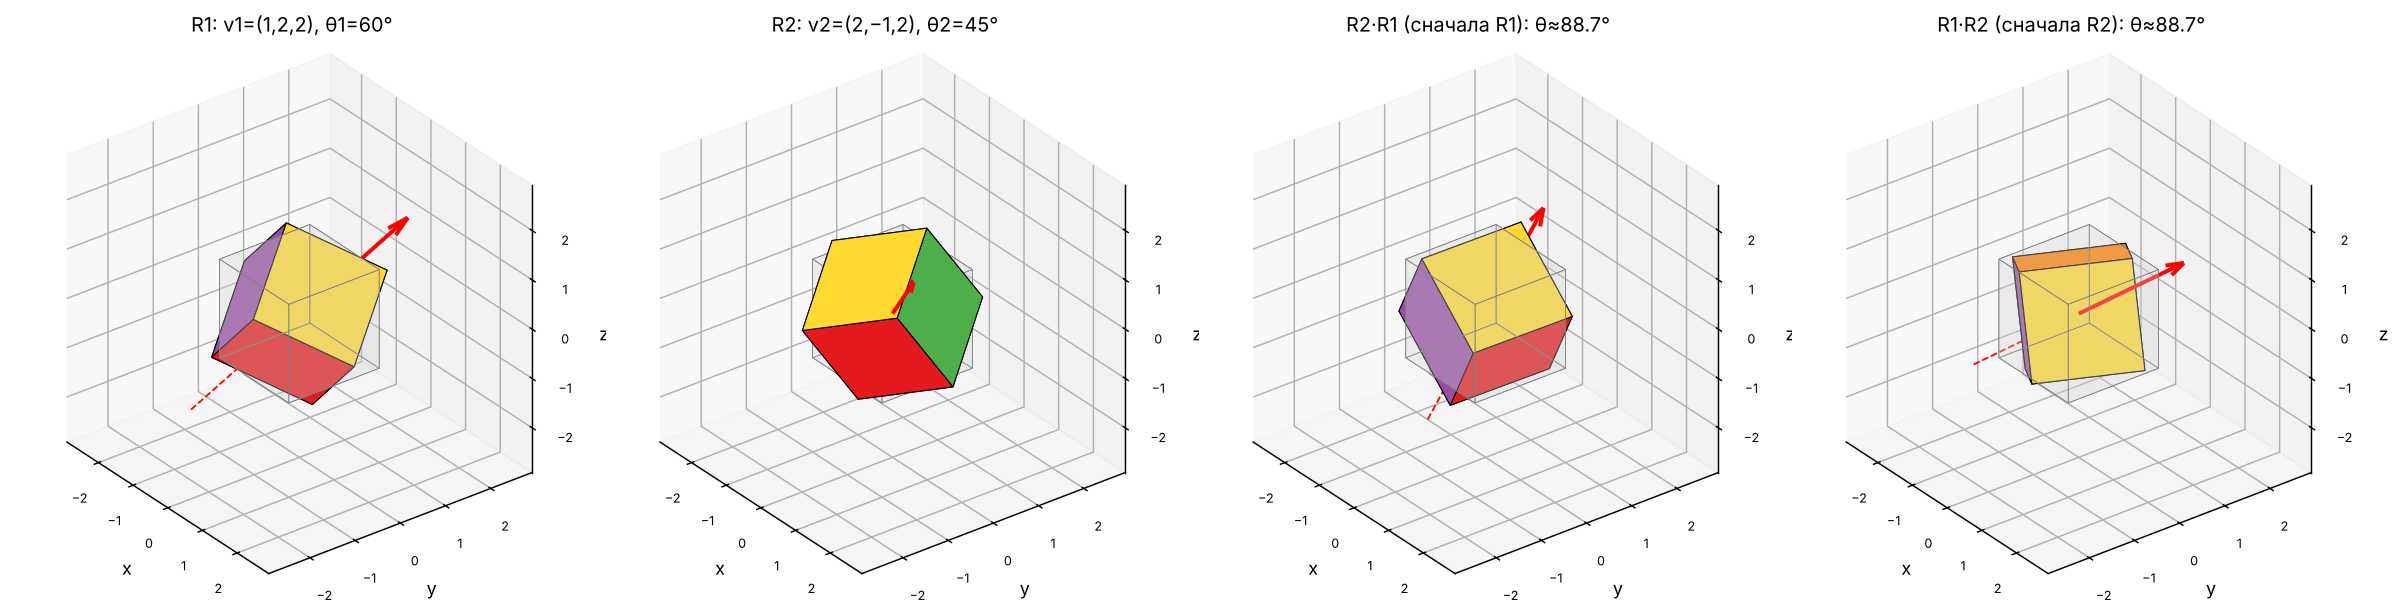
\includegraphics[width=\textwidth]{../graphics/t4_rotations.png}
        \caption{Задание 4. $R_1$, $R_2$ и композиции $R_2R_1$, $R_1R_2$ (исходный куб показан серым)}
        \label{fig:t4}
    \end{figure}
    Зависимость от угла и оси показана на рисунках~\ref{fig:t4ang} и~\ref{fig:t4ax}: при $\theta=180^\circ$ куб переворачивается ($R^2=I$), при малых $\theta$ почти не сдвигается; вращение вокруг осей $x$, $y$, $z$ оставляет неподвижным соответствующее направление.
    \begin{figure}[H]
        \centering
        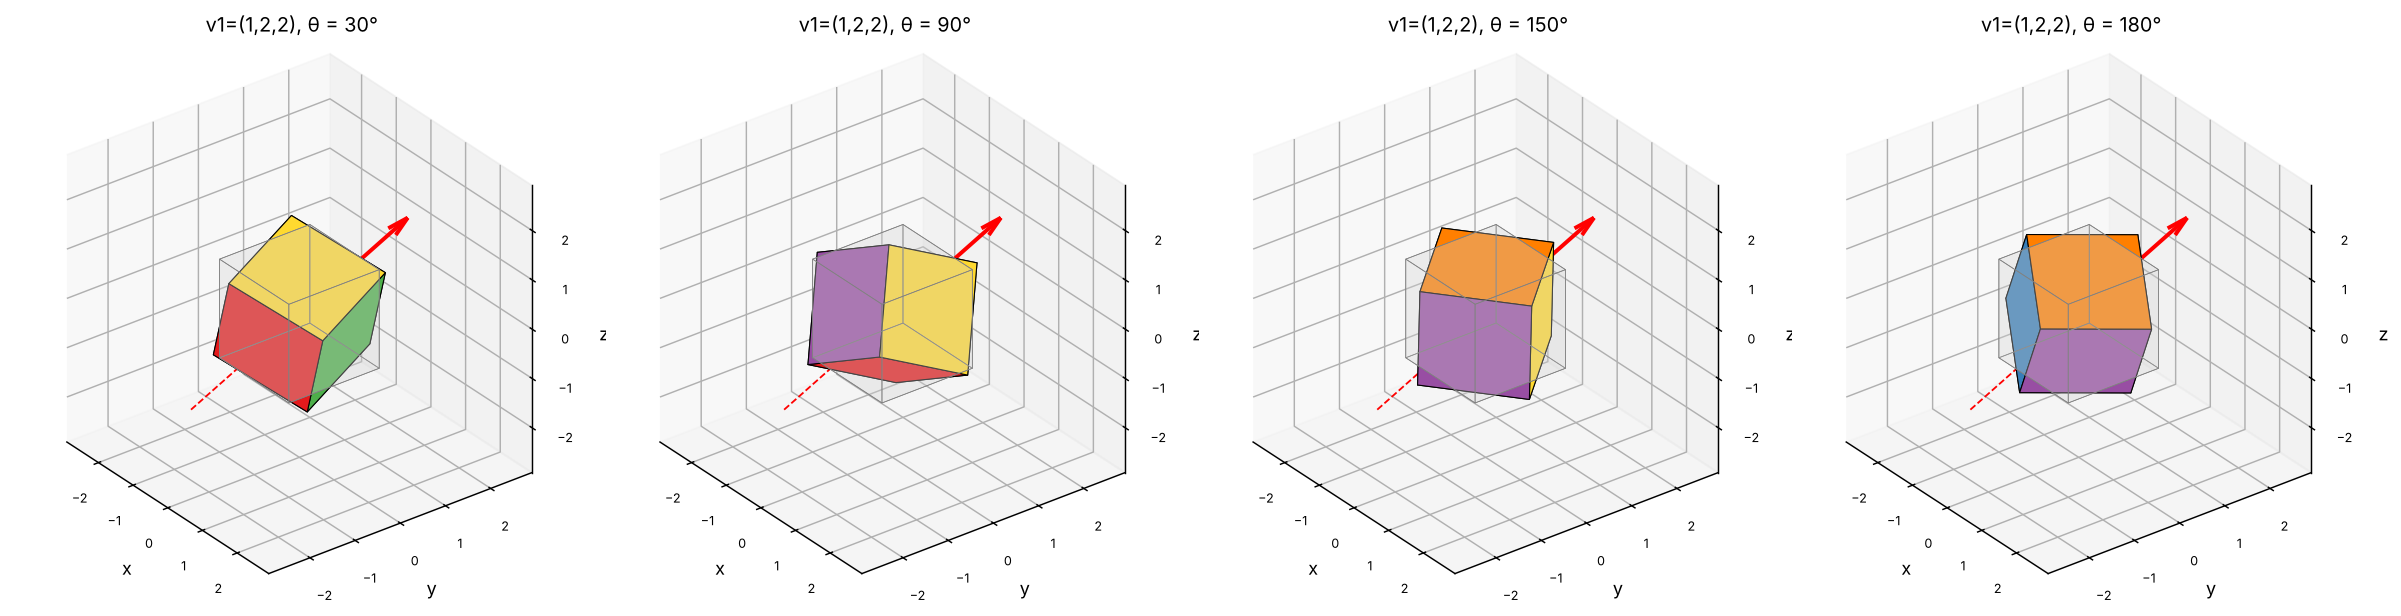
\includegraphics[width=\textwidth]{../graphics/t4_angles.png}
        \caption{Задание 4. Поворот вокруг оси $v_1$ на $30^\circ,\,90^\circ,\,150^\circ,\,180^\circ$}
        \label{fig:t4ang}
    \end{figure}
    \begin{figure}[H]
        \centering
        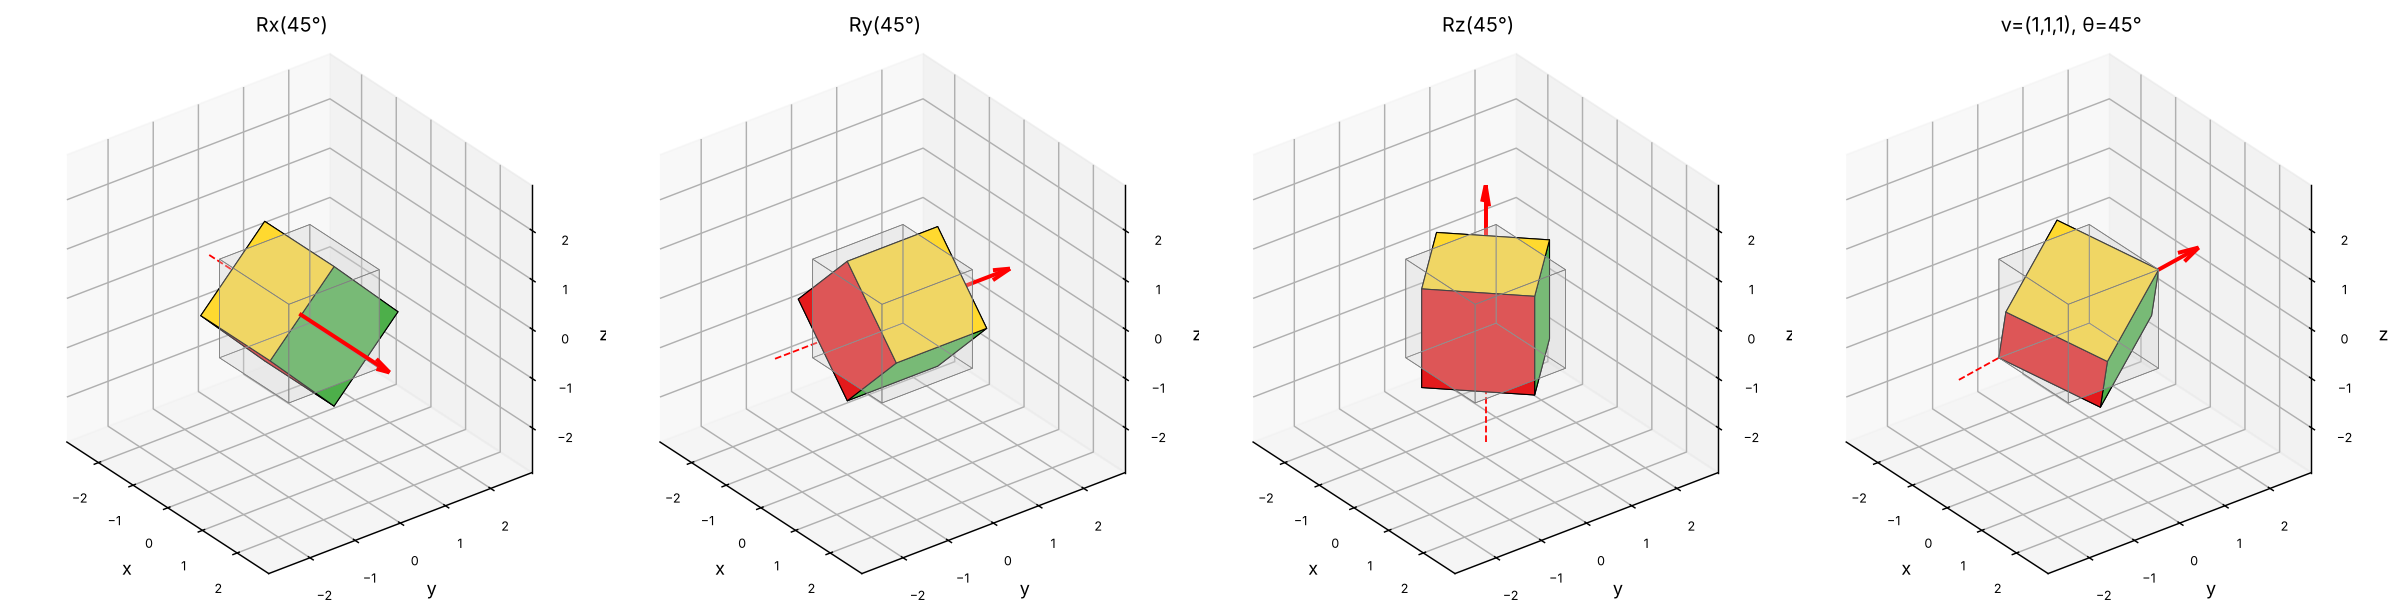
\includegraphics[width=\textwidth]{../graphics/t4_axes.png}
        \caption{Задание 4. Поворот на $45^\circ$ вокруг осей $x$, $y$, $z$ и диагонали $(1,1,1)$}
        \label{fig:t4ax}
    \end{figure}

    \section{Задание 5. Вращение вокруг вершины куба}
    \textbf{Общая формула.} Поворот вокруг оси с направлением $v$, проходящей через точку $M=(x_0,y_0,z_0)$: перенести $M$ в начало координат, повернуть вокруг $v$, вернуть назад:
    $$R_{v,M}(\theta)=T(M)\,R_v(\theta)\,T(-M)=\begin{pmatrix}R&M-RM\\0&1\end{pmatrix},$$
    где $R$ --- блок $3\times3$ матрицы $R_v(\theta)$. Точка $M$ неподвижна: $R_{v,M}M=M$.

    \textbf{Выбранное преобразование.} Центр вращения --- вершина $M=(1,1,1)$, направление оси $v=(1,1,0)^T$, угол $\theta=60^\circ$:
    $$R_{v,M}(60^\circ)=\MatRvertex.$$
    Блок $3\times3$ равен $\cos\theta I+\sin\theta J+(1-\cos\theta)\hv\hv^T$ при $\hv=(1,1,0)^T/\sqrt2$, последний столбец --- $M-RM=(-0.6124,\,0.6124,\,0.5)^T$. На рисунке красным показана ось вращения, она проходит через вершину $M$ (чёрная точка); исходный куб показан серым, повёрнутый --- цветом.
    \begin{figure}[H]
        \centering
        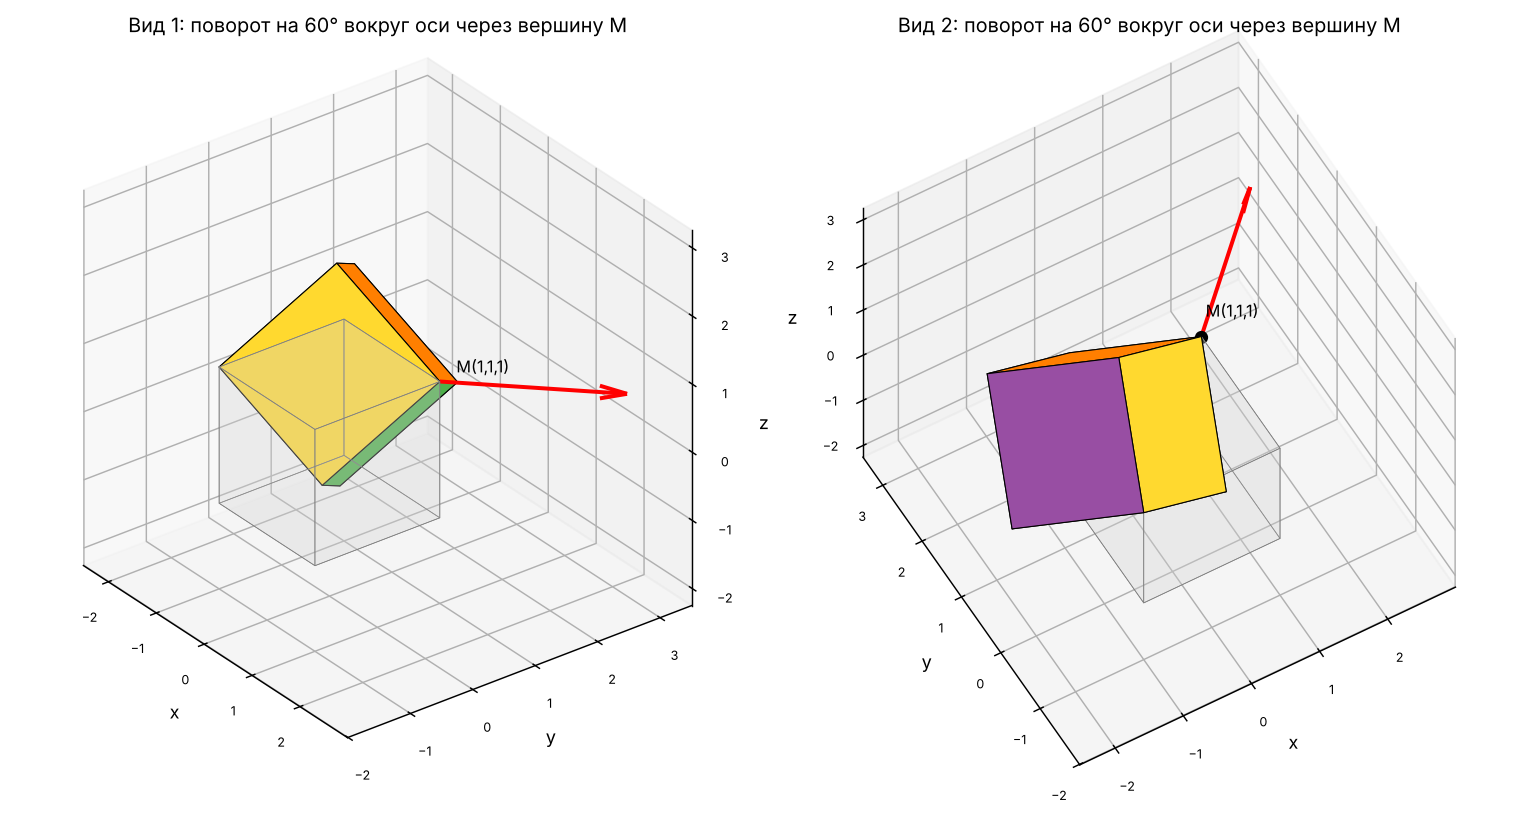
\includegraphics[width=\textwidth]{../graphics/t5_vertex_rotation.png}
        \caption{Задание 5. Исходный и повёрнутый вокруг вершины $M(1,1,1)$ куб (два ракурса)}
        \label{fig:t5}
    \end{figure}

    \section{Задание 6. Камера}
    \textbf{Сцена.} Три куба, как на рисунке~1 методички: большой голубой $T(-3,0,0)\,S(2,2,2)$; синий (единичный) в начале координат; зелёный $T(3,0,0)\,R_z(45^\circ)$. Все вершины умножаются на соответствующие матрицы. Сцена под стандартным углом камеры и при взгляде «снизу» показана на рисунках~\ref{fig:t6a} и~\ref{fig:t6b}. Для вида «снизу» использованы \texttt{ax.view\_init(azim=0, elev=-90)} и дополнительно \texttt{roll=-90}: в \texttt{matplotlib} без него ось $x$ направлена вверх, а с ним картинка совпадает с рисунком~1 методички ($x$ вправо, $y$ вниз).
    \begin{figure}[H]
        \centering
        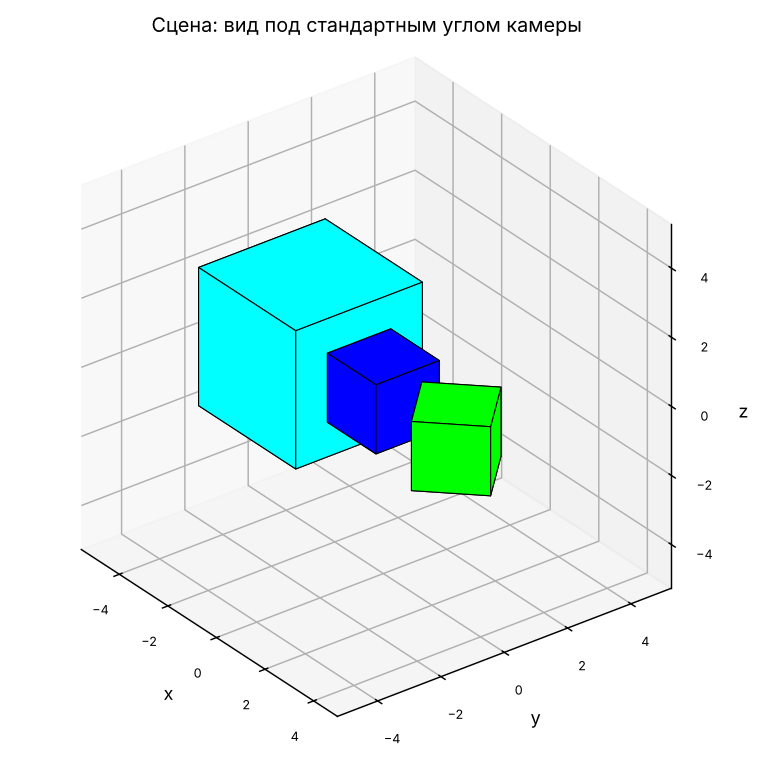
\includegraphics[width=0.48\textwidth]{../graphics/t6_scene_standard.png}\hfill
        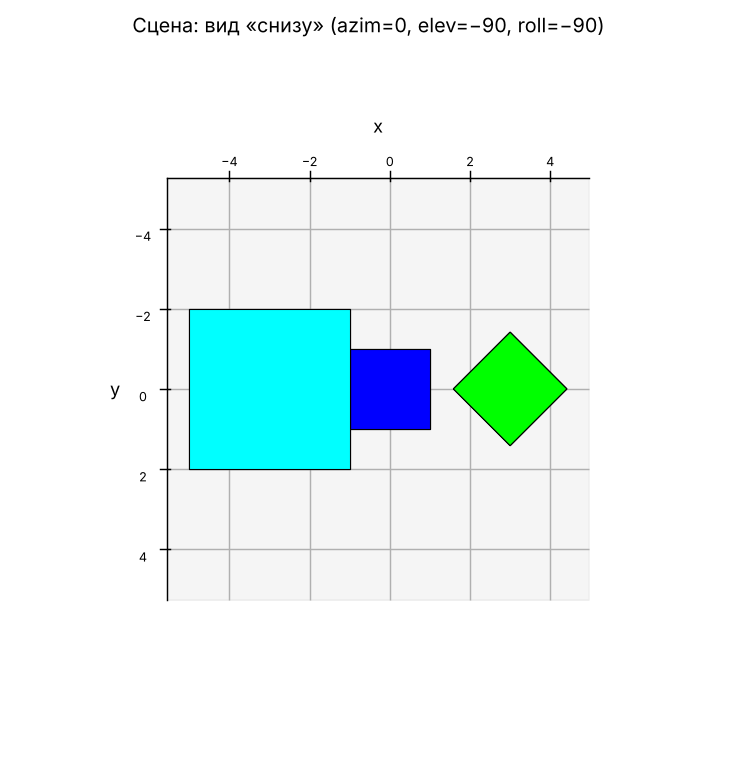
\includegraphics[width=0.48\textwidth]{../graphics/t6_scene_below.png}
        \caption{Задание 6. Сцена под стандартным углом камеры (слева) и вид «снизу» (справа)}
        \label{fig:t6a}
    \end{figure}

    \textbf{Положение камеры.} Камера описывается матрицей $C=T_cR_c$, переводящей координаты камеры в мировые: $R_c$ задаёт её поворот, $T_c$ --- положение. Выбрано $R_c=R_y(30^\circ)R_x(25^\circ)$ и расстояние $d=12$ до центра сцены, камера смотрит в начало координат (направление взгляда $R_ce_z$), то есть её положение $c=-d\,R_ce_z=\CamPos$:
    \begin{gather*}
    R_c=\MatRc,\quad T_c=\MatTc,\\
    C=T_cR_c=\MatC.
    \end{gather*}
    \textbf{Обратная матрица.} $C^{-1}=R_c^{-1}T_c^{-1}=R_c^TT(-c)$, в блочном виде $\begin{pmatrix}R_c^T&-R_c^Tc\\0&1\end{pmatrix}$:
    $$C^{-1}=\MatCinv.$$
    Проверка: $C^{-1}(c,1)^T=(0,0,0,1)^T$ (камера уходит в начало координат), а центр сцены $(0,0,0,1)^T$ переходит в $(0,0,12,1)^T$ --- на ось $z$ камеры на расстояние $d$. Применение $C^{-1}$ ко всем вершинам даёт сцену в системе координат камеры (рисунок~\ref{fig:t6c}): эта матрица --- жёсткое движение (поворот и перенос, $\det=1$), форма и размеры объектов не меняются.
    \begin{figure}[H]
        \centering
        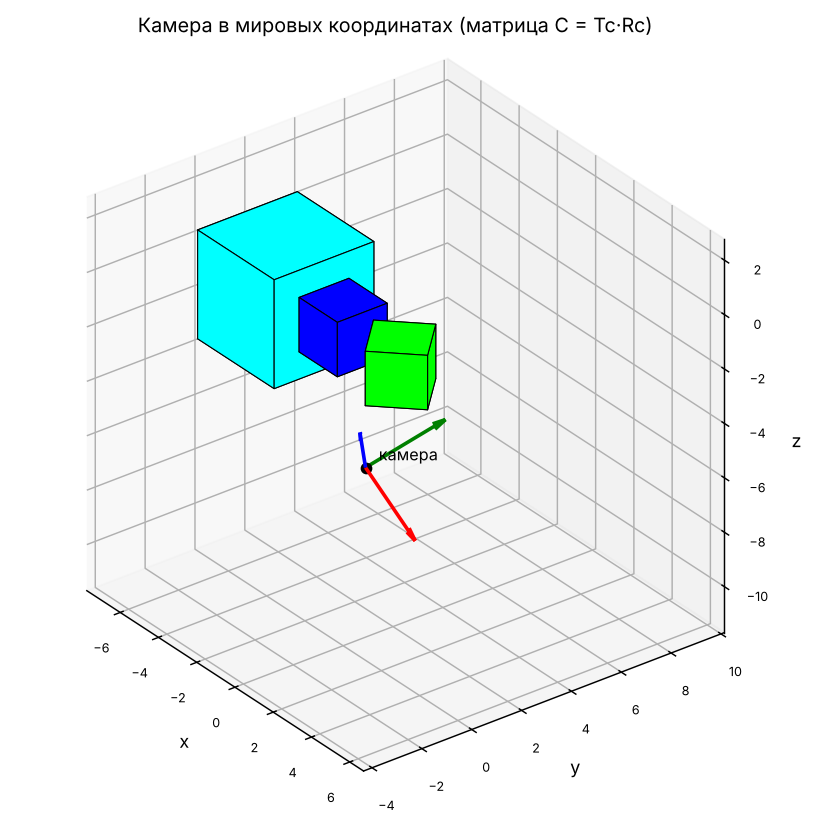
\includegraphics[width=0.48\textwidth]{../graphics/t6_camera_world.png}\hfill
        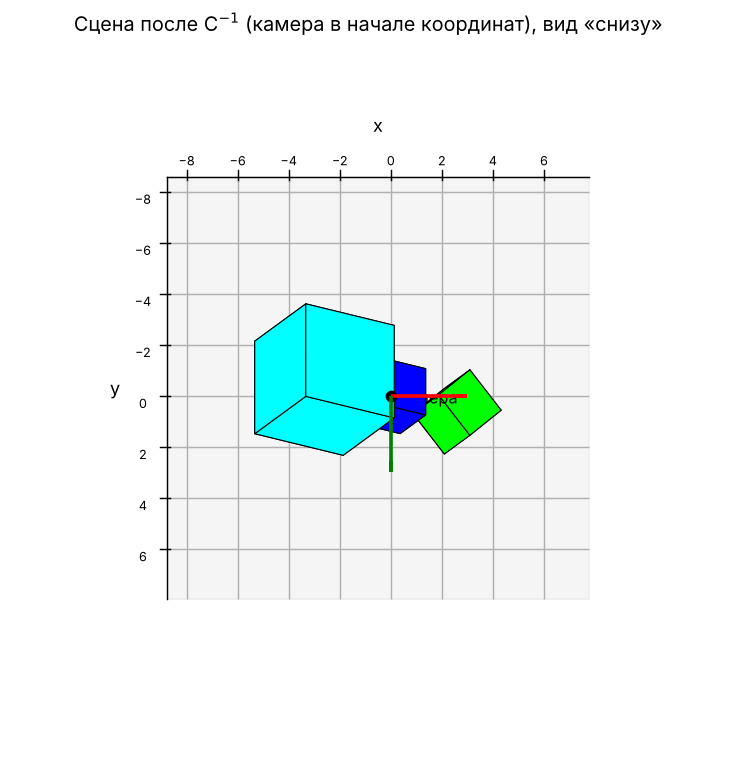
\includegraphics[width=0.48\textwidth]{../graphics/t6_scene_camera.png}
        \caption{Задание 6. Слева: камера (оси: $x$ красная, $y$ зелёная, $z$ --- направление взгляда, синяя) в мировых координатах. Справа: сцена после $C^{-1}$, вид «снизу» (с точки зрения камеры, расположенной в начале координат)}
        \label{fig:t6c}
    \end{figure}
    \begin{figure}[H]
        \centering
        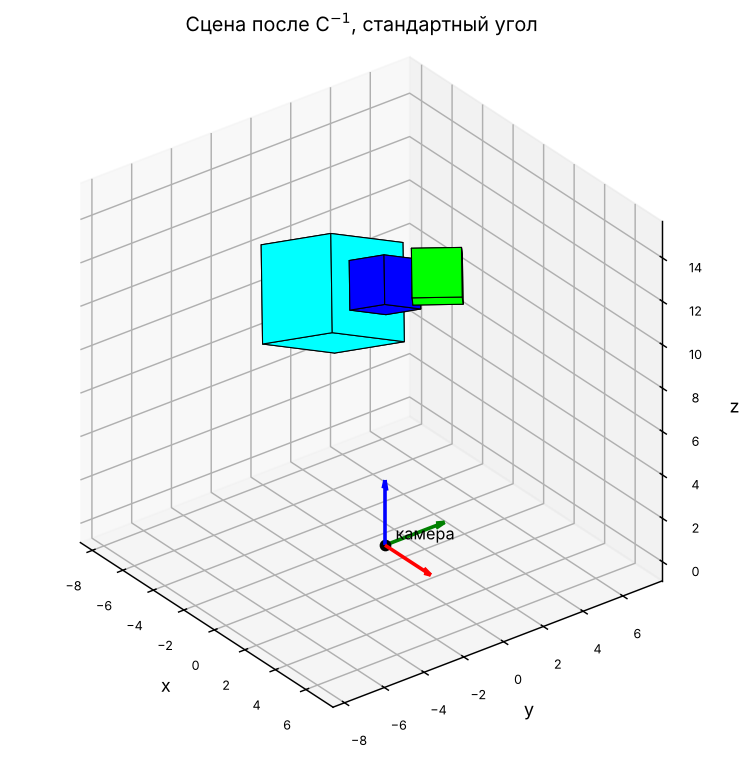
\includegraphics[width=0.6\textwidth]{../graphics/t6_scene_camera_std.png}
        \caption{Задание 6. Сцена после $C^{-1}$ под стандартным углом: видно, что сцена сдвинута вдоль оси $z$ камеры на расстояние $d=12$}
        \label{fig:t6b}
    \end{figure}

    \section{Задание 7. Перспектива}
    \textbf{Устройство матрицы.} Камера в начале координат смотрит вдоль $+z$. Видимая область --- усечённая пирамида (frustum): ближняя плоскость $z=n$ с окном $[l,r]\times[b,t]$ и дальняя плоскость $z=f$. Матрица $P$ переводит frustum в куб $[-1,1]^3$. По подобию треугольников точка $(x,y,z)$ проецируется на ближнюю плоскость в $x_p=nx/z$, $y_p=ny/z$, затем окно отображается на $[-1,1]$: $x'=\dfrac{2x_p-(r+l)}{r-l}$ и аналогично $y'$. Глубина преобразуется как $z'=A+B/z$ с условиями $z'(n)=-1$, $z'(f)=1$, откуда $A=\frac{f+n}{f-n}$, $B=-\frac{2fn}{f-n}$ (преобразование монотонно, порядок точек по глубине сохраняется). Все три формулы имеют общий знаменатель $z$, поэтому в однородных координатах
    $$P=\begin{pmatrix}\dfrac{2n}{r-l}&0&-\dfrac{r+l}{r-l}&0\\[1ex]0&\dfrac{2n}{t-b}&-\dfrac{t+b}{t-b}&0\\[1ex]0&0&\dfrac{f+n}{f-n}&-\dfrac{2fn}{f-n}\\[1ex]0&0&1&0\end{pmatrix},\qquad
    P\begin{pmatrix}x\\y\\z\\1\end{pmatrix}=\begin{pmatrix}\ast\\\ast\\\ast\\z\end{pmatrix}.$$
    Четвёртая компонента равна $z$, и деление на неё (перспективное деление) даёт $x'=\ast/z$ и т.\,д. Параметры для реализации: $n,f$ (ближняя и дальняя плоскости) и границы окна $l,r,b,t$ --- либо, для симметричного окна, угол обзора $\mathrm{FOV}$ и отношение сторон $\mathrm{aspect}$: $t=n\tan\frac{\mathrm{FOV}}2$, $r=t\cdot\mathrm{aspect}$, $l=-r$, $b=-t$. (При $r=-l$, $t=-b$ третьи элементы первых двух строк равны нулю.) Точки с $z\le0$ находятся за камерой и не имеют смысла для перспективы, поэтому все объекты должны находиться в диапазоне $n<z<f$.

    \textbf{Частный случай.} $\mathrm{FOV}=60^\circ$, $\mathrm{aspect}=1$, $n=5$, $f=25$: $t=r=5\tan30^\circ\approx2.887$,
    \begin{gather*}
    P=\MatP,\\
    \frac{2n}{r-l}=\frac{1}{\tan30^\circ}\approx1.7321,\quad \frac{f+n}{f-n}=1.5,\quad \frac{2fn}{f-n}=12.5.
    \end{gather*}
    После $C^{-1}$ вершины сцены имеют $z\in[\ZRange]\subset(5,25)$ и после $PC^{-1}$ с делением на $w$ лежат в кубе $[-1,1]^3$ (максимальная по модулю координата равна $\NDCmax$). Проверка: ближняя плоскость $z=5$ переходит в $z'=-1$, дальняя --- в $z'=+1$, угол окна $(r,t,n)\mapsto(1,1,-1)$.

    \textbf{Сравнение с изометрической камерой.} Параллельная (изометрическая, \texttt{proj\_type=\allowbreak'ortho'}) проекция просто отбрасывает координату вдоль взгляда: размер объекта не зависит от расстояния до камеры, параллельные рёбра остаются параллельными. При перспективе кубы, расположенные дальше от камеры, уменьшаются (масштаб $\sim1/z$): зелёный куб по сравнению с голубым стал заметно мельче, а рёбра, идущие вдоль взгляда, сходятся к точке схода.
    \begin{figure}[H]
        \centering
        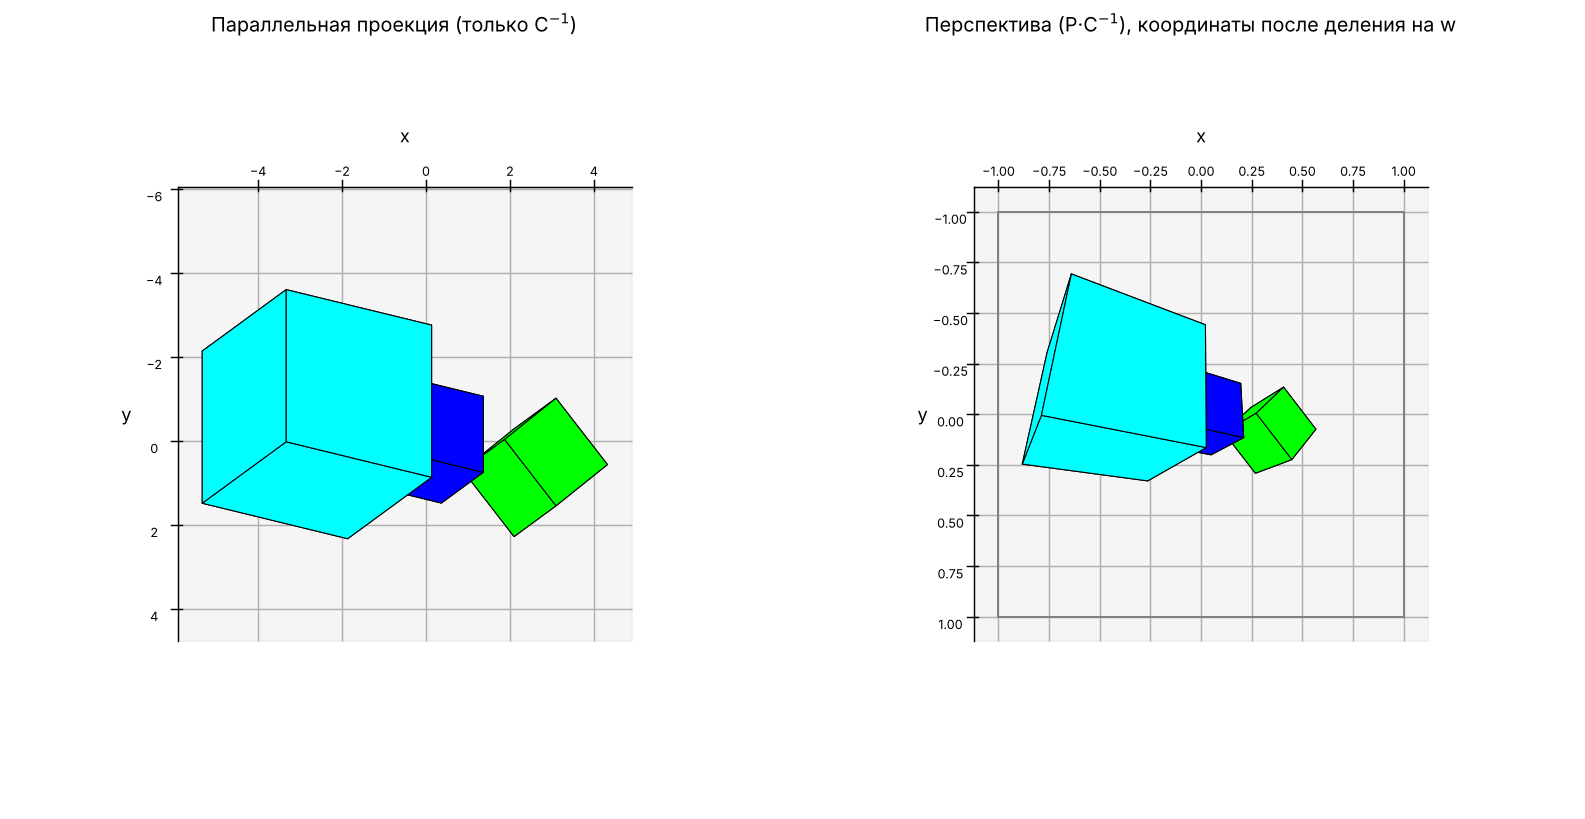
\includegraphics[width=\textwidth]{../graphics/t7_ortho_vs_persp.png}
        \caption{Задание 7. Слева: параллельная проекция (только $C^{-1}$), справа: перспектива $PC^{-1}$ после деления на $w$ (серым --- куб $[-1,1]^3$)}
        \label{fig:t7a}
    \end{figure}

    \textbf{Деформация пространства.} Рисунок~\ref{fig:t7b} показывает ту же сцену до и после $P$ в одном ракурсе: пирамида видимости превращается в куб, сходящиеся рёбра пирамиды становятся параллельными оси $z$, а объекты ближе к камере растягиваются (сильнее по $z$), дальше --- сжимаются. Рисунок~\ref{fig:t7c} --- вращение стандартной камеры (\texttt{view\_init}) для пространства после перспективы: видно, что расстояние по глубине распределено неравномерно (дальние объекты сильно сжаты по $z'$), а сами кубы деформируются в усечённые пирамиды.
    \begin{figure}[H]
        \centering
        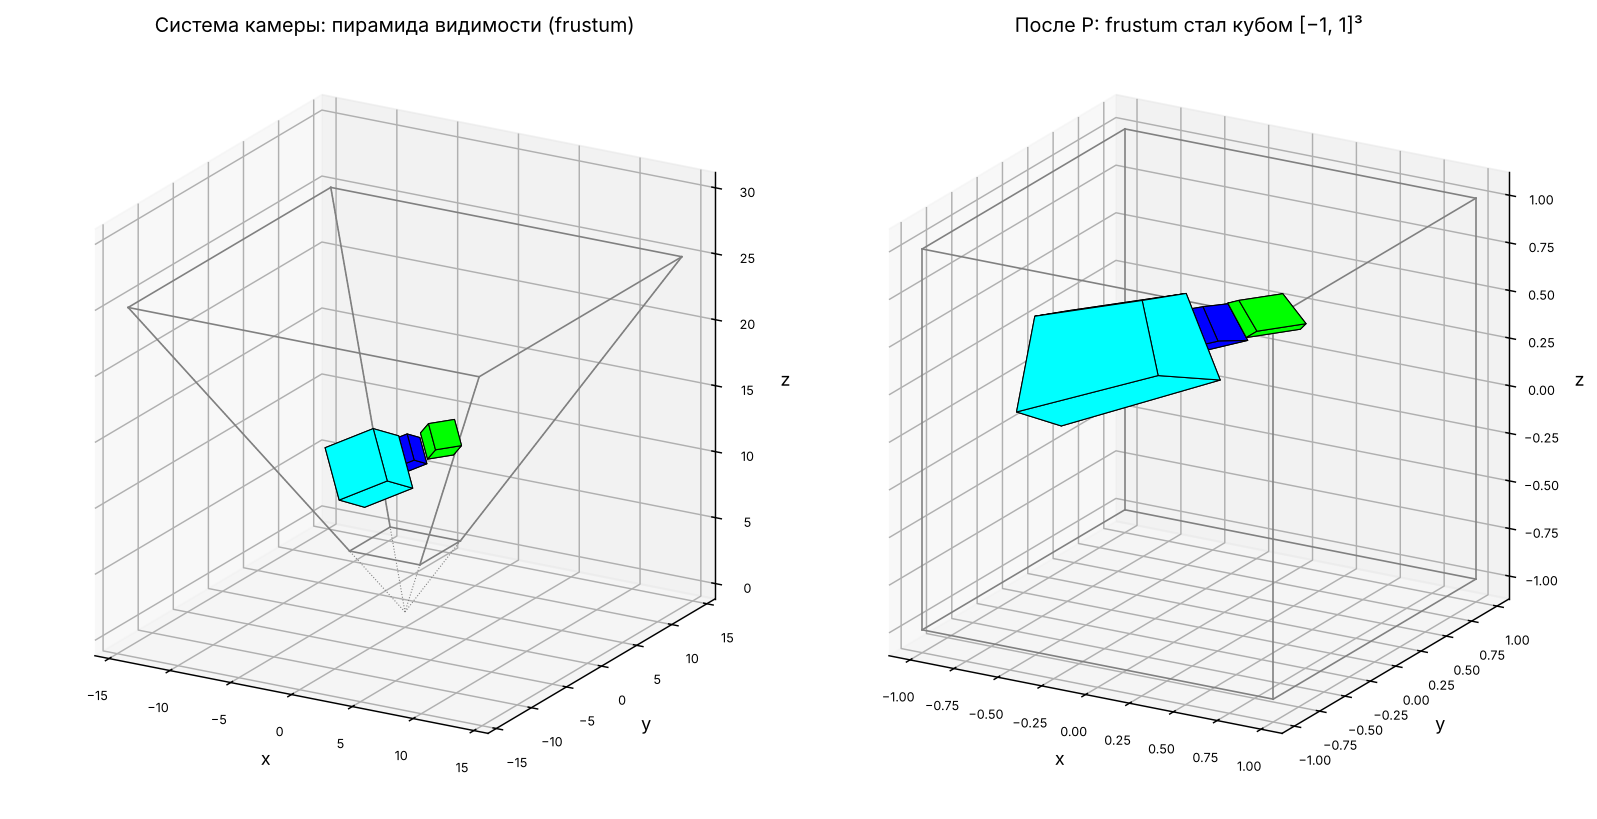
\includegraphics[width=\textwidth]{../graphics/t7_frustum_to_cube.png}
        \caption{Задание 7. Слева: сцена в системе камеры с пирамидой видимости ($n=5$, $f=25$, $\mathrm{FOV}=60^\circ$). Справа: та же сцена после $P$ --- пирамида стала кубом $[-1,1]^3$}
        \label{fig:t7b}
    \end{figure}
    \begin{figure}[H]
        \centering
        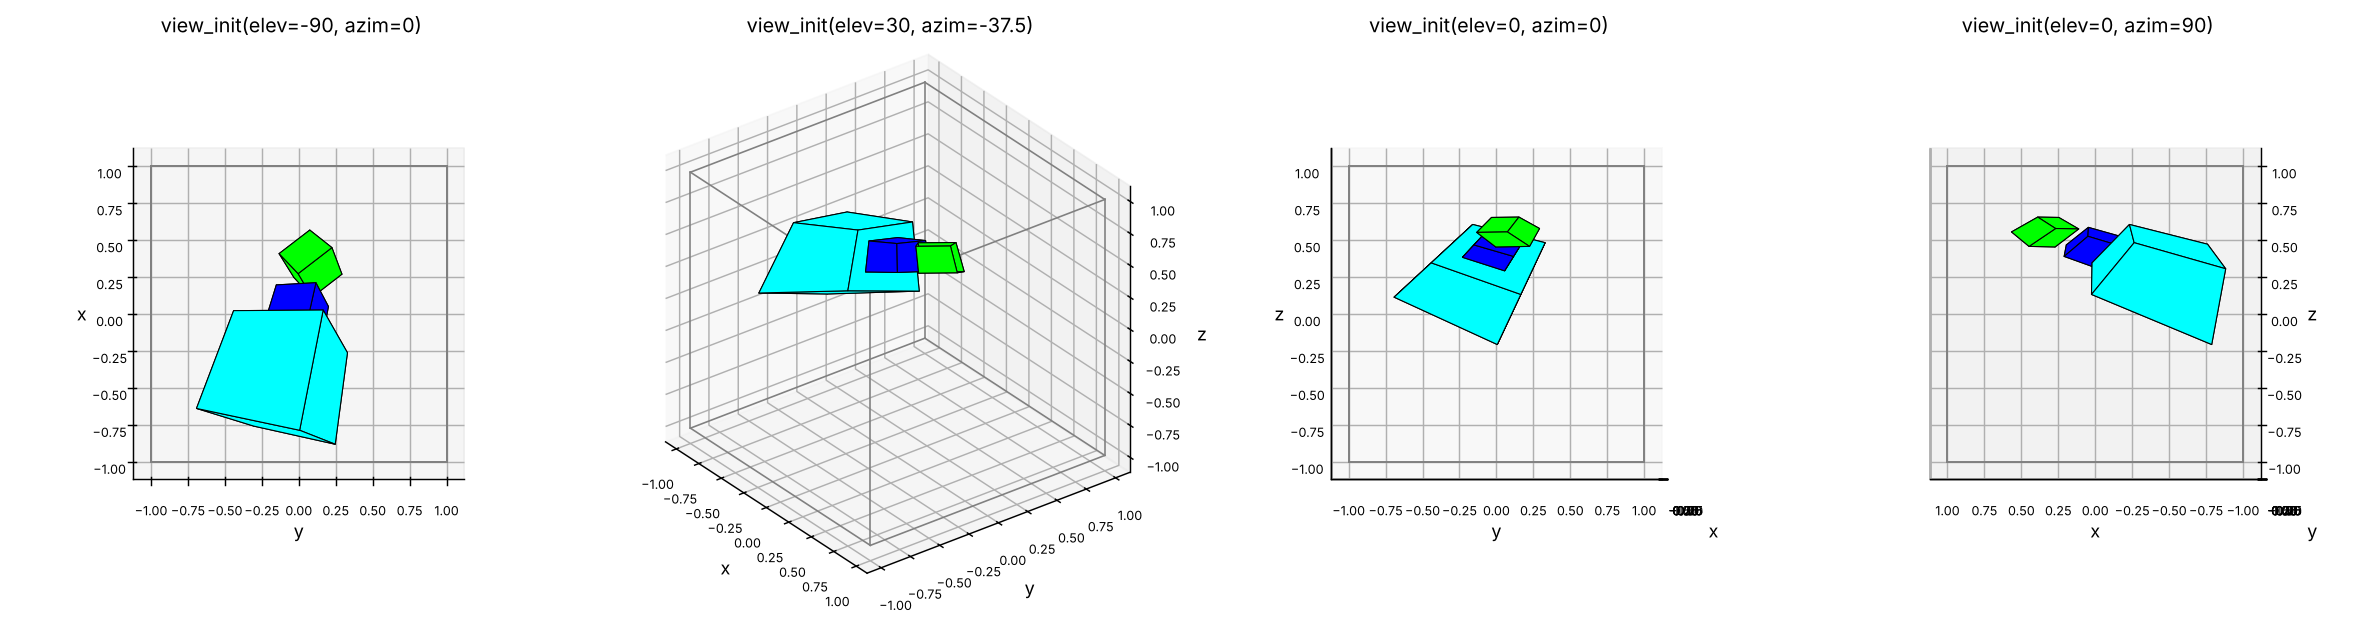
\includegraphics[width=\textwidth]{../graphics/t7_views.png}
        \caption{Задание 7. Пространство после перспективы под разными углами: \texttt{view\_init(elev=-90, azim=0)} (с \texttt{roll=-90}), \texttt{(30, -37.5)}, \texttt{(0, 0)}, \texttt{(0, 90)}}
        \label{fig:t7c}
    \end{figure}

    \section{Задание 8 (необязательное). Домик}
    Домик построен из блоков, каждый получен матрицами масштабирования, поворота и перемещения из куба или призмы (в виде $T\,R\,S\,V$): стены --- $T(0,0,1.5)\,S(2.5,2,1.5)$ от куба; крыша --- $T(0,0,3)\,S(2.8,2.3,1.3)$ от треугольной призмы (вершины $4\times6$, грани: два треугольника и три четырёхугольника); труба --- $T(1.5,0.8,3.8)\,S(0.3,0.3,0.8)$; дверь и два окна --- тонкие параллелепипеды на передней стене; сарай рядом --- $T(5.5,-0.5,0.75)\,R_z(30^\circ)\,S(1,1,0.75)$ с крышей из призмы; зелёная земля --- плоский четырёхугольник. Камера направлена на домик сверху и спереди: $c=(-9,-13,9)$, взгляд в точку $(0.5,0,1.5)$, ось $y$ камеры направлена вниз (против $z$ мира), так что домик на виде «снизу» стоит правильно. Для неё
    $$C=T_cR_c=\MatCh,$$
    $C^{-1}$ применяется ко всем объектам, затем перспектива $\mathrm{FOV}=60^\circ$, $n=5$, $f=40$:
    $$P=\MatPh.$$
    Слева на рисунке --- мировые координаты, посередине --- вид параллельной камеры, справа --- перспектива (углы домика сходятся, сарай, находящийся дальше, мельче).
    \begin{figure}[H]
        \centering
        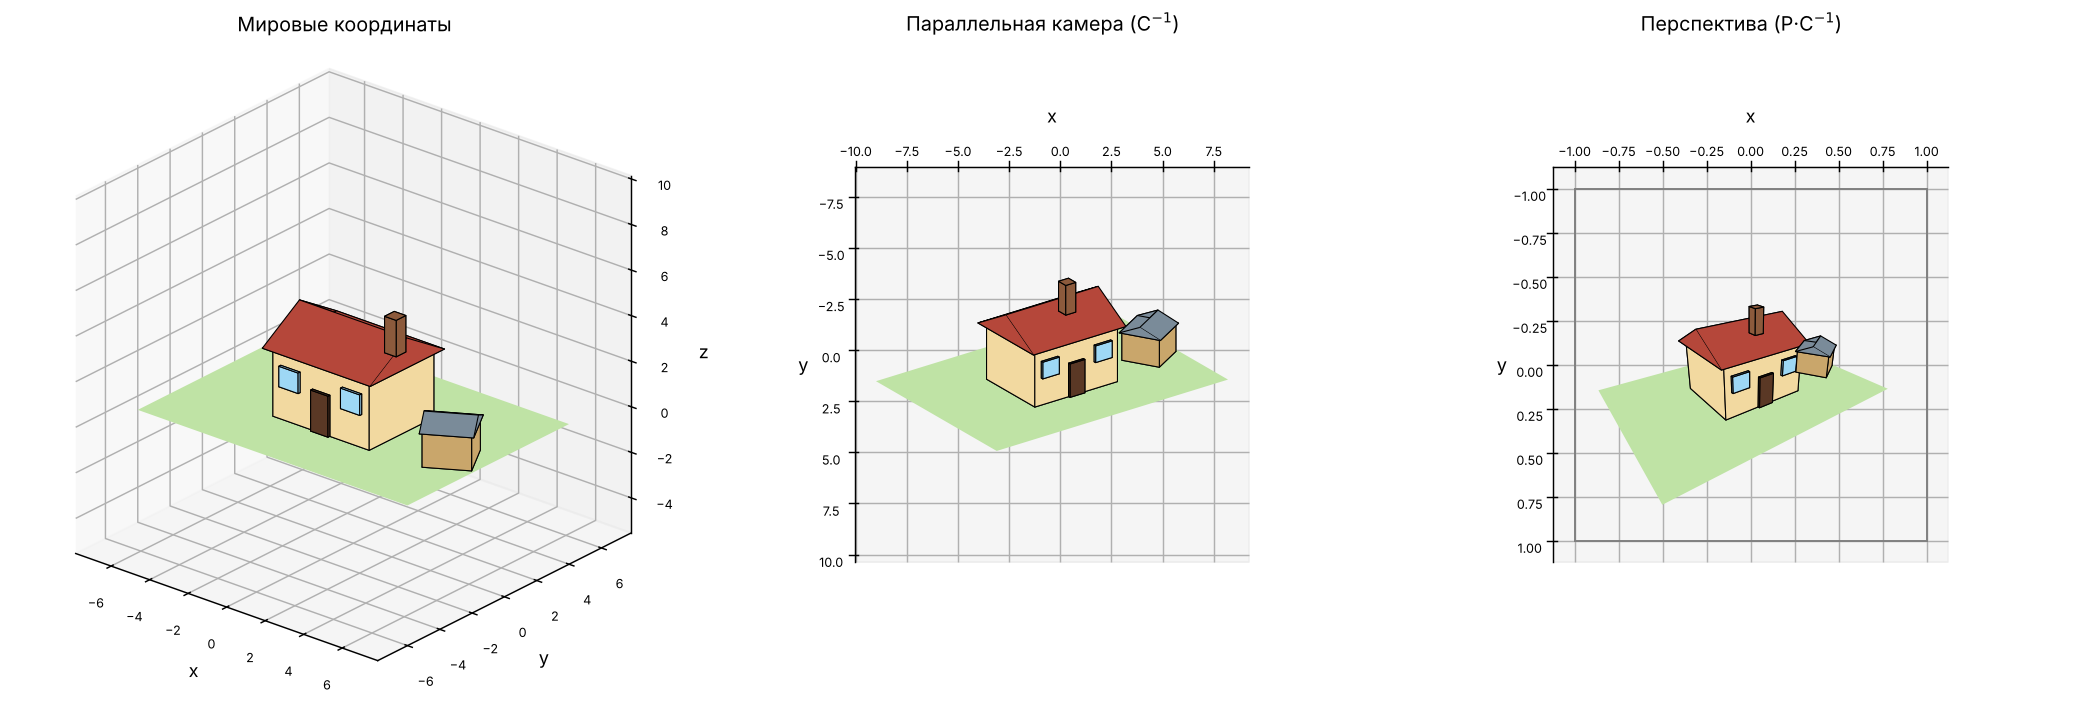
\includegraphics[width=\textwidth]{../graphics/t8_house.png}
        \caption{Задание 8. Домик: мировые координаты, параллельная камера $C^{-1}$ и перспектива $PC^{-1}$}
        \label{fig:t8}
    \end{figure}

    \section{Выводы}
    Все геометрические преобразования (масштабирование, перенос, поворот, смена камеры, перспектива) записаны матрицами $4\times4$ в однородных координатах, поэтому их композиция --- обычное умножение матриц, причём порядок существенен: $TS\neq ST$, $R_2R_1\neq R_1R_2$. Матрица поворота $R_v(\theta)=e^{J\theta}$ строится из кососимметрической матрицы векторного произведения, является ортогональной и оставляет неподвижной ось; поворот вокруг точки $M$ --- это сопряжение $T(M)R_vT(-M)$. Матрица камеры $C^{-1}$ --- жёсткое движение, переносящее камеру в начало координат; перспектива $P$ нелинейна в $\mathbb R^3$, но линейна в однородных координатах, и после деления на $w=z$ превращает пирамиду видимости в куб. Правильность матриц проверена в программе численно (ортогональность, совпадение $\exp$ с формулой Родрига, неподвижность осей и центра вращения, образы ближней и дальней плоскостей).

    \section{Приложение. Код выполнения}
\lstinputlisting[caption={Программа построения матриц и визуализации}, label={lst:code}]{../prog/main.py}

\end{document}
